
\section{Background and motivations}
\label{sec:background}

This section introduces the general outline of the random peer sampling
protocols. Then, it details two state-of-the-art approaches that will be used
later on. Finally, we highlight the motivations of our approach.

\subsection{Random peer sampling}
Random peer sampling protocols provide each peer with a partial view
$\mathcal{P}$ of the network membership $N$. The partial views are populated
with a uniform distribution of randomly chosen peers. A wide variety of
gossip-based protocols use random peer sampling (e.g. topology management
(REF)). Nonetheless, providing each peer with a uniform random sample relying
solely on local knowledge remains challenging.  Our Scamplon protocol is based
on two state-of-the-art approaches, namely Scamp and Cyclon.

%% Talk about Cyclon
\begin{asparadesc}
\item [Cyclon] is a periodic random peer sampling protocol which updates its
  partial view every interval of time. The partial view has a fixed-size set at
  start. In this view, each neighbour is associated with an age incremented at
  each cycle. To update its partial view, Cyclon exchanges a subset of its
  partial view with one of its neighbour chosen by using the age. The exchange
  guarantees that the network graph stays connected.
\end{asparadesc}

%% Talk about Scamp
\begin{asparadesc}
\item [Scamp] stands for SCalable Membership Protocol. It is a reactive
  protocol which provides each membership event with an appropriate reaction.
  %% add moar on scamp properties
  Figure~\ref{fig:scampexample} depicts the joining protocol of Scamp. As we
  can see, the resulting graph is connected. However, the last peer $p_1$ only
  has one neighbour in its partial view, meaning that if $p_4$ crashes, $p_1$
  cannot send messages to the network any more. To avoid that, a periodic
  re-subscription is necessary.
\end{asparadesc}

\begin{figure}
  \centering
  
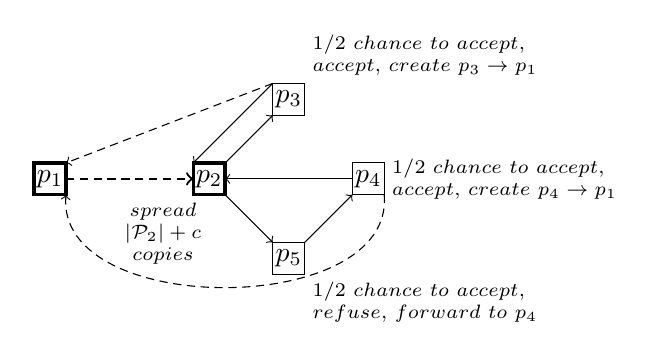
\begin{tikzpicture}[scale=1.15]
  
  \draw[fill=white, very thick] (0pt, 0pt)
  node{$p_1$} +(-5pt,-5pt) rectangle +(5pt,5pt);

  \begin{scope}[shift={(75pt,0pt)}]
  \draw[fill=white, very thick]
  (-25pt, 0pt) node{$p_2$} +(-5pt,-5pt) rectangle +(5pt,5pt);
  \draw[fill=white] (0pt,  25pt) node{$p_3$} +(-5pt,-5pt) rectangle +(5pt,5pt);
  \draw[fill=white] ( 25pt, 0pt) node{$p_4$} +(-5pt,-5pt) rectangle +(5pt,5pt);
  \draw[fill=white] (0pt, -25pt) node{$p_5$} +(-5pt,-5pt) rectangle +(5pt,5pt);


  \draw[->] (-20pt, 5pt) -- (-5pt, 20pt); 
  \draw[->] (-20pt,-5pt) -- (-5pt,-20pt); 
  \draw[->] ( 5pt,-20pt) -- (20pt, -5pt); 
  \draw[->] (20pt,  0pt) -- (-20pt, 0pt); 
  \draw[->] (-5pt, 30pt) -- (-30pt, 5pt); 

  \draw[->, thick, densely dashed] (-70pt, 0pt) -- (-30pt, 0pt); 
  \draw[->, densely dashed] (-5pt, 30pt) -- (-70pt, 5pt); 
  \draw[->, densely dashed] (30pt, -5pt)to[out=-85,in=-95](-70pt,-5pt);

  \scriptsize
  \draw (-25pt,-5pt) node[align=center,anchor=north east]
  {$spread$\\$|\mathcal{P}_2|+c$\\$copies$};
  \draw (5pt,-30pt) node[align=left,anchor=north west]
  {$1/2$ $chance$ $to$ $accept,$\\$refuse,$ $forward$ $to$ $p_4$};
  \draw (5pt, 30pt) node[align=left,anchor=south west]
  {$1/2$ $chance$ $to$ $accept,$\\$accept,$ $create$ $p_3 \rightarrow p_1$};
  \draw (30pt, 0pt) node[align=left,anchor=west]
  {$1/2$ $chance$ $to$ $accept,$\\$accept,$ $create$ $p_4 \rightarrow p_1$};
  \end{scope}
  
%%  \small
%%  \begin{scope}[shift={(130pt,0pt)}]
%%    \draw[fill=white](5pt, 0pt)node{$p_x$}+(-5pt,-5pt) rectangle +(5pt,5pt);
%%    \draw (10pt,0pt) node[anchor=west]{Peer $p_x$};
%%    \draw[->](0pt, -12pt)--(10pt, -12pt) node[anchor=west]{Established link};
%%    \draw[->, densely dashed](0pt, -19pt)--(10pt, -19pt)
%%    node[anchor=west]{New link};
%%    
%%  \end{scope}
  
\end{tikzpicture}
  \caption{\label{fig:scampexample} Scamp's joining protocol on a small
    network. Peer $p_1$ wants to join $p_4$'s network composed of $p_2$,
    $p_3$, $p_4$, and $p_5$. Peer $p_1$ establishes a connection to $p_4$. Then
    $p_4$ copies $|\mathcal{P}|$-times the new subscription and sends one to
    each neighbour. To handle possible failures, $c$ additionnal copies (here
    $0$ for simplicity sake), are sent to random neighbours. Then, each peer
    has a probability of $1\over{|\mathcal{P}|+1}$ to accept the forwarded
    subscription, hence, to establish a connection to reach $p_1$. Otherwise,
    the peer forwards it to another peer in $\mathcal{P}$ at random. Here,
    $p_3$ accepts the subscription, $p_2$ forwards it to $p5$, and the latter
    accepts it. The resulting graph is connected.}
\end{figure}

\subsection{Motivations}
%% Talk about motivations
In this paper, we do not restrict ourself to the one-way connections. Instead,
we also study the effect of three-way handshake connection set-up. 


%%% Local Variables:
%%% mode: latex
%%% TeX-master: "../paper"
%%% End:
